\documentclass[tikz]{standalone}

\usepackage{circuitikz}

\begin{document}
	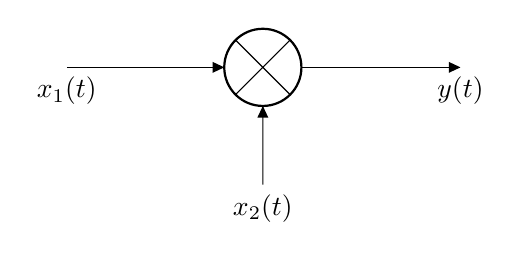
\begin{tikzpicture}
		\draw (0,0) node[below]{$x_1(t)$} (2,0)
            node[mixer, anchor=west](mixer){};
		\draw (0,0) to[short] (mixer.west);
        \node [inputarrow, anchor=tip] at (mixer.west) {};
        \draw (mixer.east) to[short] (5,0) node[inputarrow]{} node[below]{$y(t)$};
        \draw (mixer.south) to[short] ++(0,-1) node[below]{$x_2(t)$};
        \node [inputarrow, anchor=tip, rotate=90] at (mixer.south) {};
	\end{tikzpicture}
\end{document}